\documentclass[12pt, letterpaper]{article}
\usepackage{geometry}
\geometry{
 a4paper,
 total={170mm,257mm},
 left=20mm,
 top=20mm,
 }
\usepackage{graphicx} % Required for inserting images
\usepackage[english,greek]{babel}
\usepackage{mathabx} % Load the mathabx package
\usepackage{subcaption}

\newcommand{\en}{\selectlanguage{english}}
\newcommand{\gr}{\selectlanguage{greek}}


\graphicspath{{../plots/}} % specify the path to the images

\title{Εργασία Θεωρίας Δικτύων }
\author{Φίλιππος Ρωσσίδης \\ (ΑΕΜ 10379)}
\date{\today}


\begin{document}
\maketitle

\section{Εισαγωγή}

Στην εργασία αυτή εξετάζουμε την αναγνώρηση κοινοτήτων. Συγκεκριμένα θα 
υλοποιούμε την 
\textlatin{distance quality function}  θα ελέγξουμε κατά πόσο αυτή είναι καλή
επιλογή. 

Οι συναρτήσεις αυτές (\textlatin{quality functions}) δέχονται ως όρισμα έναν
γράφο και μια κατανομή κοινοτήτων και επιστρέφουν μία τιμή. Σκοπώς μας είναι 
να επιστρέφουν υψηλές τιμές για κατανομές που παρουσιάζουν ισχυρή κοινοτική συμπεριφορά,
ώστε να μπορούμε μεγιστοποιώντας αυτή τη συνάρτηση να ανιχνεύσουμε τις κοινότητες.

Θα υλοποιηθεί η συνάρτηση με έναν βέλτιστο ως προς τη ταχύτητα τρόπο, όπως και δύο αλγόριθμοι μεγιστοποίησής της. Θα υλοποιηθούν 
και κάποια \textlatin{benchmarks} ώστε να ποσοτικοποιηθεί η απόδοσή της και θα συγκριθεί με την εδραιωμένη μετρηκότητα \textlatin{modularity}.


\section{Η συνάρτηση \textlatin{distance quality}}

\subsection{Μαθηματικός Ορισμός}

Η συνάρτηση δέχεται σαν όρισμα έναν γράφο και κάποια κατανομή κοινοτήτων.

Ορίζουμε:

\[ D_V(i,j) = \min \{ k:A^k_G (i,j) \neq 0 \} \]
τον πίνακα που περιέχει τις αποστάσεις μεταξύ κάθε δύο κόμβων του γράφου 
$i,j$, όπου $A^k_G(i,j)$ ο πίνακας γειτνίασης του γράφου $G$. υψομένος στην $k$
δύναμη. 

Ορίζουμε επίσης:
\[ D_V(c) = \sum_{i,j \in c} D_V(i,j) \]

Αυτό αποτελεί μέτρο του πόσο στενά συνδεδεμένες είναι μεταξύ τους 
οι κοινότητες. Επιθυμούμε να το συγκρίνουμε με την αναμενώμενη τιμή 
για τυχαίο γράφο.

Για να ορίσουμε τον τυχαίο γράφο επιλέγουμε το γενικευμένο μοντέλο,
όπου συνδέουμε τυχαία ακμές μεταξύ κόμβων, διατηρώντας όμως τον βαθμό τους.


Αν $d_k(v)$ είναι ο $k$ βαθμός του κόμβου $v$, δηλαδή το πλήθος των 
ελάχιστων μονοματιών μήκους $k$ που ξεκινάν από τον $v$ και 
$m_k(G) = \frac{1}{2} \sum_{v \in V (G)} d_k(v)$ το πλήθος 
ελάχιστων μονοπατιών μήκους $k$ στον γράφο $G$, τότε η πιθανότητα δύο κόμβοι
$i,j \in G$ να συνδέονται με ακμή μήκους $k$ είναι:
\[ Pr[i,j,k] = \frac{d_k(i)}{2m_k(G)} \frac{d_k(j)}{2m_k(G)} \]
η αναμενώμενη απόσταση των κόμβων:
\[ \overline{D_V(i,j)} = \sum_{k=1}^{diam(G)} k Pr[i,j,k] \]
όπου $diam(G)$ η διάμετρος του γράφου (μέγιστο ελάχιστο μονοπάτι).

Αν ορίσουμε
\[ \overline{ D_V(c)  } = \frac{1}{2} \sum_{i,j \in c} \overline{ D_V(i,j) }\]
το άθροισμα των αναμενώμενων αποστάσεων των κόμβων στην κοινότητα $C$, 
τότε η συνάρτηση:

\[ Q_d(G,C) = \sum_{c \in C} (\overline{ D_V(c) } - D_V(c))\]
δηλώνει την επιθυμητή σύγκριση του μέτρου στενής σύνδεσης των κοινοτήτων 
$C$ ως προς του τυχαίου γράφου. 

Περιμένουμε οι τιμές της $Q_d$ να είναι υψηλές για ισχυρές δομές κοινοτήτων.


Στην υλοποίηση μου διάλεξα επίσης να τροποποιήσω την συνάρτηση ως εξίς:

\[ D_V(c) = \sum_{i,j \in c} D_V(i,j) \]
\[ \overline{ D_V(c)  } =  \sum_{i,j \in c} \overline{ D_V(i,j) }\]
\[ Q_d(G,C) = \sum_{c \in C} [(1 - \gamma)\overline{ D_V(c) } - \gamma D_V(c) ],  \ \ \ \ \gamma \in (0,1)\]

ώστε για $\gamma = 0.5$ να ισοδυναμεί με τον προϋγούμενο ορισμό, αλλά να έχω 
δυνατότητα να επιλέξω ποιός όρος θα επηρρεάσει περισσότερο.



\subsection{Υλοποίηση}


Χρησιμοποιήθηκε δυναμική προσέγγιση, δηλαδή οι τιμές του αλγορίθμου που χρησιμοποιούνται 
συχνά ($D_V(i,j), \ d_k(i), \ m_G(k), \ Pr[i,j,k],  \ \overline{D_V(i,j)},..$)
υπολογίζονται μία φορά στην αρχή και αποθηκεύονται ώστε να καλούνται σε σταθερό χρόνο στην πορεία. Έτσι γλυτώνουμε τις 
άσκοπες επαναλύψεις. Ειδικότερα στην περίπτωση του συγκεκριμένου αλγορίθμου, αφού 
η συνάρτηση ποιότητας θα υπολογιστεί χιλιάδες φορές για διαφορετικές 
επιλογές κοινοτήτων στην διαδικασία μεγιστοποίησής της, και εφόσον οι μακράν 
πιο αργές διαδικασίες (όπως θα περιγραφτεί παρακάτω) είναι αυτές των 
προαναφερθέντων ποσοτήτων, η διαφορά στο χρόνο εκτέλεσης είναι ραγδαία. 

Όπου είναι δυνατό χρησιμοποιούνται συναρτήσεις της βιβλιοθήκης $networkx$ μιας και 
είναι βελτιστοποιημένες και θα συμβάλουν στην ταχύτητα του κώδικα.

Στην πρώτη φάση του αλγορίθμου υπολογίζονται οι παρακάτω ποσότητες και αποθηκεύονται
για μελλοντική χρήση:
\begin{itemize}
    \item \textbf{διάμετρος του γράφου } 
    
    Χρησιμοποιείται η συνάρτηση της βιβλιοθήκης $networkx: diameter(G)$.
    
    \item  $\mathbf{D_V(i,j)}$
    
    Χρησιμοποιείται η συνάρτηση της βιβλιοθήκης $networkx: all\_pairs\_shortest\_path\_length(G)$,
    η οποία επιστρέφει απευθείας το ζητούμενο, την απόσταση κάθε δύο κόμβων του γράφου
    μεταξύ τους. Τα στοιχεία αποθηκεύονται σε ένα $python \ dict$. Η χρονική
    πολυπλοκότητα της συνάρτησης αυτής είναι $O(|V|^2\log |V| +|V||E|)$ (?), όπου 
    $|V|$ το πλήθος κόμβων του γράφου και $|E|$ το πλήθος των ακμών. 


    \item  $\mathbf{d_k(i)}$ \ και \ $\mathbf{m_G(k)}$
    
    Χρησιμοποιείται η συνάρτηση της βιβλιοθήκης $networkx:$ \\
    $ singe\_source\_shortest\_path\_length(G,source)$, η οποία υπολογίζει για κάποιον
    κόμβο $source$ όλα τα ελάχιστα μονοπάτια που τον έχουν σαν άκρο. Αν υπολογιστούν 
    αυτά τα μονοπάτια για κάθε κόμβο ως $source$ τότε θα έχουμε υπολογίσει
    όλα τα ελάχιστα μονοπάτια του γράφου δύο φορές (μία για $i \rightsquigarrow j$ και 
    μια για $j \rightsquigarrow i$). Η συνάρτηση χρησιμοποιεί την τεχική 
    $Breadth \ First \ Search$, έτσι η χρονική πολυπλοκότητα της είναι 
    $O(|V|+|E|)$

    Τρέχουμε την παραπάνω συνάρτηση για κάθε κόμβο του γράφου ($source$). Στο $dict$ που 
    αυτή επιστρέφει, περιέχονται για κάθε άλλο κόμβο  ($target$) μια λίστα με μήκη από όλα
    τα μονοπάτια που τους ενώνουν ($source \rightsquigarrow target$). Έτσι για κάθε 
    μονοπάτι που βρίσκουμε στη λίστα, έχουμε το μήκος του $k$, 
    αυξάνουμε κατά $1$ τον βαθμό $d_k(source)$ και κατά $0.5$ τη τιμή 
    $m_G(k)$. Χρησιμοποιούμε $0.5$ διότι $m_k(G) = \frac{1}{2} \sum_{v \in V (G)} d_k(v)$
    (μετράμε κάθε μονοπάτι $2$ φορές).

    Η  πολυπλοκότητα της παραπάνω διαδικασίας είναι: $\#add complexity$.

    \item $\mathbf{Pr[i,j,k]}$  \ και \   $\mathbf{\overline{D_V(i,j)}}$
    
    Υπολογίζονται απλά με τους τύπους:
    \[ Pr[i,j,k] = \frac{d_k(i)}{2m_k(G)} \frac{d_k(j)}{2m_k(G)} \]
    \[ \overline{D_V(i,j)} = \sum_{k=1}^{diam(G)} k Pr[i,j,k] \]
    και αποθηκεύονται. 
    
    Συγκεκριμένα οι πίνακες αυτοί είναι συμμετρικοί (αφού 
    $\frac{d_k(i)}{2m_k(G)} \frac{d_k(j)}{2m_k(G)} = \frac{d_k(j)}{2m_k(G)} \frac{d_k(i)}{2m_k(G)}$)
    οπότε οι τιμές αυτές υπολογίζονται μία φορά για κάθε ζευγάρι $i,j$ και προστίθονται
    στο τέλος μία φορά για $i=j$ και δύο για $i \neq j$.
    
    Η χρονική πολυπλοκότητα της παραπάνω διαδικασίας είναι:
    $\#add complexity$.

    

\end{itemize}

Προσοχή χρειάζεται το γεγονός ότι οι παραπάνω διαδικασίες δε μπορούν 
να λειτουργήσουν για μη συνδεδεμένους γράφους. Έτσι υιοθετούμε τη σύμβαση ότι 
δύο μη συνδεδεμές συνεκτικές συνιστώσες δεν μπορούν να βρίσκονται στην ίδια 
κοινότητα. Όποτε διαχωρίζουμε τον γράφο στις συνεκτικές του συνιστώσες και 
τρέχουμε τα παραπάνω για κάθε μία ξεχωριστά. Αυτή η προσέγγιση διατηρεί την 
πολυπλοκότητα ίδια (αφού οι συνεκτικές συνιστώσες διαμερίζουν τον γράφο).

\bigskip

\emph{Συνολική πολυπλοκότητα της πρώτης φάσης: $add complexity$.}

\bigskip

Στη δεύτερη φάση του αλγορίθμου, αφού έχουν αποθηκευτεί τα παραπάνω, 
υπολογίζονται για τις δοσμένες κοινότητες $C$ τα αθροίσματα: 


\[ D_V(C) = \sum_{i,j \in C} D_V(i,j), \qquad \overline{ D_V(C)  } =  \sum_{i,j \in C} \overline{ D_V(i,j) }\]
 για $i,j \in C$, και η τιμή:
\[ Q_d(G,C) = \sum_{c \in C} [(1 - \gamma)\overline{ D_V(C) } - \gamma D_V(C) ]\]


\bigskip

\emph{Συνολική πολυπλοκότητα της δεύτερης φάσης: $O(|V|^2)$.}

\bigskip







\subsubsection{Μια πρώτη ματία στα αποτελέσματα}



\begin{figure}
  \begin{subfigure}{0.5\textwidth}
    \centering 
    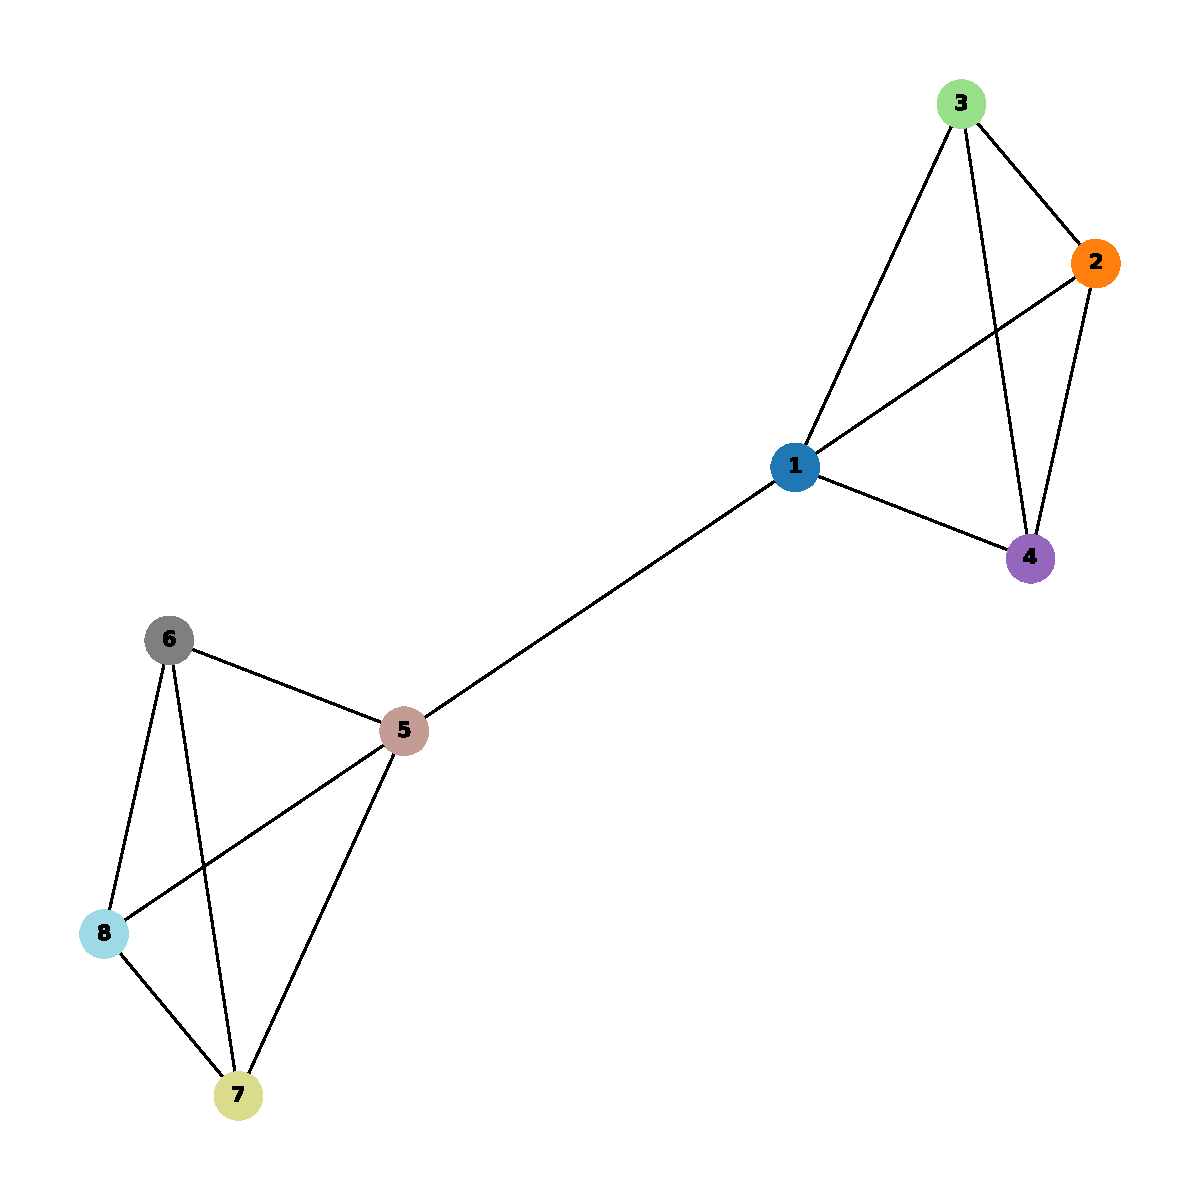
\includegraphics[width=0.5\linewidth]{quad_comm_gamma=0.5.pdf}
    \caption{Αποτελέσματα ωμής δύναμης για $\gamma = 0.5$. Κάθε κόμβος βρίσκεται σε δική του κοινότητα.}
    \label{fig:graph8comm}
  \end{subfigure}
  \begin{subfigure}{0.5\textwidth}
    \centering 
    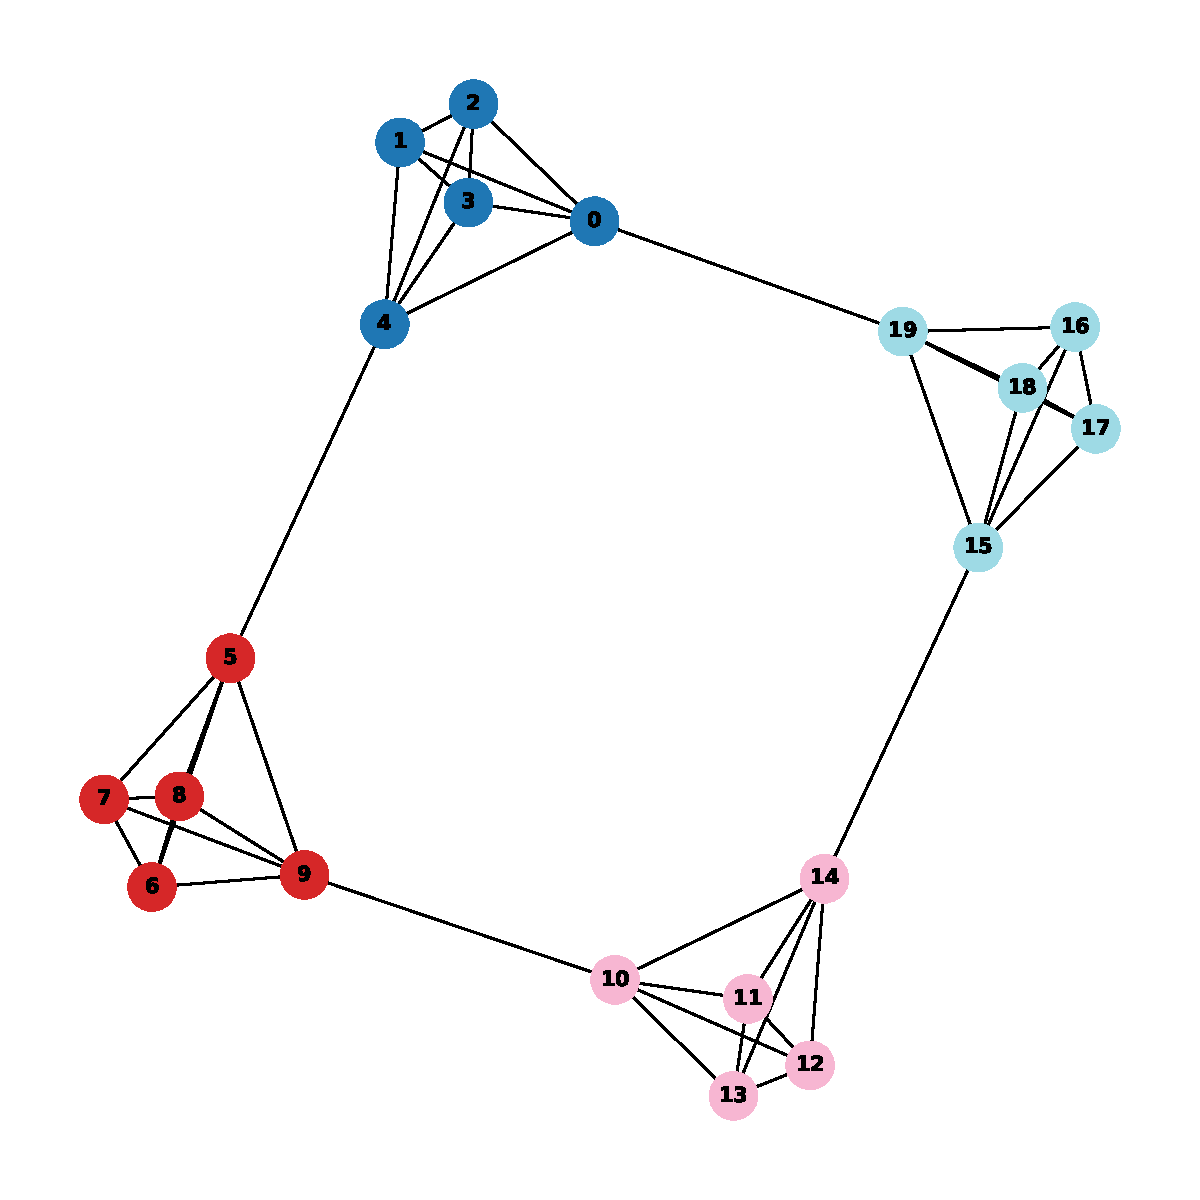
\includegraphics[width=0.7\linewidth]{cluster_4,5gamma=0.02,newman.pdf}
    \caption{Αποτελέσματα αλγορίθμου \textlatin{Newman} για $\gamma = 0.02$. Οι κοινότητες έχουν αναγνωριστεί σωστά.}
    \label{fig:newman4,5}
  \end{subfigure}
\end{figure}



Για μια πρώτη εικόνα της λειτουργίας της παραπάνω μετρηκής, δοκιμάστηκε τεχνική ωμής δύναμης σε διάφορους γράφους,
για $\gamma = 0.5$ (δηλαδή τον αρχικό ορισμό της).
Ένα παράδειγμα βρίσκεται στο σχήμα \ref{fig:graph8comm}, όπου κάθε κοινότητα χρωματίζεται με δικό της χρώμα. 

Στο σχήμα φαίνονται οι κοινότητες για τις οποίες η τιμή $Q_d$ είναι μέγιστη. Ενώ περιμέναμε για τον γράφο αυτό να επιστραφούν 
δύο κοινότητες των 4 κόμβων, βλέπουμε ότι αυτό δεν συμβαίνει. Συγκεκριμένα για $\gamma = 0.5$ βρέθηκε πειραματικά ότι 
τη μέγιστη τιμή $Q_d$ παίρνουμε πάντα όταν κάθε κόμβος έχει δική του κοινότητα. Σε αυτό θα χρησιμεύσει η τιμή $\gamma$, όπου με την 
αλλαγή της μπορούμε να έχουμε τη επιθυμητή συμπεριφορά.

Παρατίθεται προκαταβολικά στο σχήμα \ref{fig:newman4,5} το αποτέλεσμα του αλγορίθμου \textlatin{Newman} για $\gamma = 0.02$ για να φανεί 
το γεγονός αυτό.















\section{Αλγόριθμοι μεγιστοποίησης του $Q_d$}



\subsection{Πρώτη προσπάθεια άπληστου αλγορίθμου}

Θα περιγράψω τον πρώτο αλγόριθμο που υλοποιήθηκε συνοπτικά, διότι παρότι αντικαταστάθηκε 
από αυτόν του \en Newman, \gr παρουσιάζει κάποια διαφορά στην λογική και τα αποτελέσματα:

\begin{enumerate}
  \item Υπολογίζουμε τις απαραίτητες ποσότητες και τις αποθηκεύουμε \\ ($D_V(i,j), \ d_k(i), \ m_G(k), \ Pr[i,j,k],  \ \overline{D_V(i,j)},diam(G)$).
  \item Αρχικοποιούμε κάθε κόμβο σε δική του κοινότητα.
  \item Για κάθε κόμβο, υπολογίζουμε τον γειτονικό του κόμβο στου οποίου την κοινότητα 
  εάν μεταφερθεί θα υπάρει η μέγιστη μεταβολή στο $Q_d$. Εάν η μεταβολή αυτή είναι θετική,
  τότε τον μεταφέρουμε σε εκείνη την κοινότητα.
  \item Επαναλαμβάνουμε το βήμα 3 μέχρι να μην γίνεται καμία μεταβολή.
\end{enumerate}

Ο αλγορίθμος αυτός δέχεται βελτιστοποίηση, 







\subsection{\textlatin{Newman}}

Για καλύτερα αποτελέσματα υλοποιήθηκε ο αλγόριθμος που προτάθηκε από τον \textlatin{Newman} 
\cite{Newman}\relax. 

Ο αγλόριθμος αυτός προτάθηκε για τη μεγιστοποίηση της \en modularity, \gr αλλά μπορεί με τις κατάλληλες τροποποιήσεις να χρησιμοποιηθεί και εδώ.

Στον αλγόριθμο ξεκινάμε με μια κοινότητα για κάθε κόμβο και ενώνουμε διαδοχικά τις κοινότητες οι οποίες θα έχουν μέγιστη αύξηση του $Q$. Μετά από $|V|-1$ συνδέσεις
θα έχει μείνει μόνο μία κοινότητα, όποτε απαιτούνται το πολύ $|V|-1$ συνδέσεις. 

Στην ταχύτητα βοηθάει η παρατήρηση ότι δε χρειάζεται να υπολογίζεται συνέχεια η τιμή της $Q_d$ αλλά μόνο η διαφορά $\Delta Q_d(c_i,c_j)$ της $Q_d$ αν συνενώσουμε τις 
κοινότητες $c_i$ και $c_j$. 


Περιγραφικά:

Έστω ότι έχω κοινότητες $C = {c_1,..,c_n}$ και συνενώνω τις κοινότητες $c_i,c_j \in C$ ώστε να αποκτήσω
στο επόμενο βήμα κοινότητες $C'$. Έστω επίσης ότι $Q_d$ είναι η τιμή της \textlatin{distance quality}
στις κοινότητες $C$, ενώ $Q_d'$ στις $C'$. 



Για ευκολία συμβολίζω: 
\[ I(c) = [(1 - \gamma)\overline{ D_V(c) } - \gamma D_V(c)] \]
και,
\[ J(i,j) = (1-\gamma) \overline{ D_V(i,j)} - \gamma D_V(i,j) \]
τότε,
\[ Q_d = \sum_{c \in C} I(c) =\sum_{c \in C} \sum_{i,j \in c} J(i,j) \]
Έχουμε:
\[ Q_d  = \sum_{c \in C} I(c) =  \sum_{c \in C \setminus c_i,c_j}[I(c)] + I(c_i) + I(c_j) \Leftrightarrow\]
\[ Q_d = \sum_{c \in C \setminus c_i,c_j}[I(c)] + \sum_{i,j \in c_i}J(i,j) + \sum_{i,j \in c_j}J(i,j)  \]
καi,
\[ Q_d' = \sum_{c \in C'} I(c) =  \sum_{c \in C \setminus c_i,c_j}[I(c)] + I(c_i \cup c_j) \Leftrightarrow \]
\[ Q_d' =  \sum_{c \in C \setminus c_i,c_j}[I(c)] + \sum_{i,j \in c_i \cup c_j} J(i,j) \]



Από τα παραπάνω είναι φανερό ότι:
\[   \Delta Q = Q_d' - Q_d = 2 \sum_{i \in c_i, j \in c_j} J(i,j) \Leftrightarrow \]
\[ \Delta Q = 2 \sum_{i \in c_i, j \in c_j} (1-\gamma) \overline{ D_V(i,j)} - \gamma D_V(i,j) \]



Στον συγκεκριμένο αλγόριθμο διατηρώ έναν πίνακα $\Delta Q$ ο οποίος στη θέση $i,j$ περιέχει τη διαφορά $\Delta Q_d (c_i,c_j)$. 
Σε κάθε βήμα βρίσκω το μέγιστο στοιχείο του πίνακα και ενώνω τις κοινότητες αυτές $c_i,c_j$. Σύμφωνα με τη παρατήρηση των 
\en Clauset-Newman-Moore \gr \cite{Clauset:fastgreedy} όταν γίνει το $max \Delta Q$ πρώτη φορά αρνητικό, γνωρίζουμε ότι από εκεί και πέρα θα συνεχίσει
να είναι αρνητικό, ή η $Q_d$ θα συνεχίσει να μειώνεται. Επομένως δεν έχει σημασία η αναζήτηση πέραν αυτού του σημείου και ο αλγορίθμος σταματάει όταν 
βρει $max \Delta Q \leq 0$. 
 
Καλύτερα ||| Ίσως $v,u$ στις κοινότητες..

\[ \Delta Q = 2 [ (1 - \gamma)   \overline{ D_V(i,j)}- \gamma D_V(i,j) ]\]



Όταν ενώσω $c_i,c_j$ στην $j$ πως αλλάζει ο $\Delta Q$:

για κάθε $c_k \in C$
\[ \Delta Q_{jk} = 2 \sum_{i \in c_i \cup c_j, j \in c_k} J(i,j) = 2 \sum_{i \in c_i, j \in c_k} J(i,j) + 2 \sum_{i \in c_j, j \in c_k} J(i,j) = \Delta Q_{ik} + \Delta Q_{jk}\]




\selectlanguage{english}
\renewcommand{\refname}{\selectlanguage{greek} Αναφορές}  
\bibliographystyle{plain}
\bibliography{sources.bib}



\end{document}
